\newpage
\subsubsection{ALS Chain}
\textit{ALS Chains} sind die Verallgemeinerung von \textit{ALS XZ} und \textit{ALS XY Wing}. Ein \textit{ALS XZ} ist eine \textit{ALS Chain} der Länge 2 und ein \textit{ALS XY Wing} ist eine \textit{ALS Chain} der Länge 3. Eine \textit{ALS Chain} ist eine Kette von {ALS} verbunden durch \textit{RCCs}, für die gilt, dass keine zwei aufeinanderfolgenden \textit{RCCs} gleich sein dürfen. Die \textit{ALS} am Anfang und Ende der Kette enthalten eine gemeinsame Ziffer Z. Diese Ziffer wird wie gewohnt dann aus allen Kandidatenlisten gelöscht, die von allen Instanzen der Ziffer Z im \textit{ALS} am Anfang und am Ende der Kette gesehen werden.\\
Das geht, da durch die Verknüpfung durch \textit{RCCs} die Ziffer Z entweder im \textit{ALS} am Anfang der Kette stehen muss oder in dem am Ende.

\begin{figure}[h]
\begin{center}
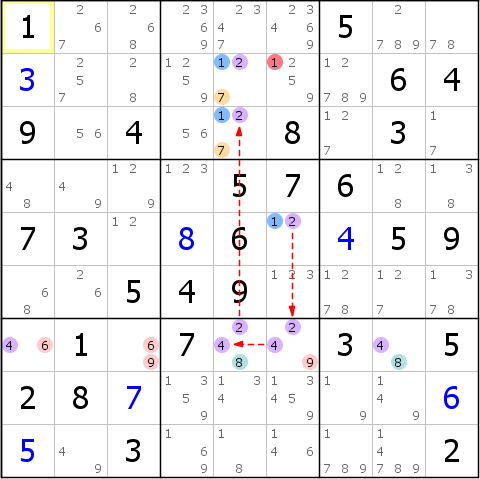
\includegraphics{./img/ALS_Chain.png}
\caption{ALS Chain}
\end{center}
\end{figure}

In \textbf{Abbildung 2.22} sieht man eine \textit{ALS Chain} der Länge 4. Das erste und einzellige \textit{ALS} ist in z5s6, es enthält die Kandidaten 1 und 2. Durch den \textit{RCC} 2 ist es verbunden mit dem\textit{ALS} in Zeile 7 Spalten 1, 3 und 6, das die Kandidaten 2, 4, 6 und 9 enthält. Dieses \textit{ALS} ist durch den \textit{RCC} 4 verbunden mit dem \textit{ALS} in Zeile 7, Spalten 5 und 8 mit den Kandidaten 2, 4 und 8. Die letzte Verbindung besteht dann durch den \textit{RCC} 2 zum \textit{ALS} in Spalte 5 Reihen 2 und 3, es enthält die Kandidaten 1, 2 und 7. Das erste und das letzte \textit{ALS} enthalten den gemeinsamen Kandidaten 1. Dieser kann nun als Kandidat aus allen Zellen gelöscht werden, die alle Instanzen der Ziffer 1 in beiden \textit{ALS} sehen. Das ist der Fall in z2s6.